\begin{figure}[htbp]\centering
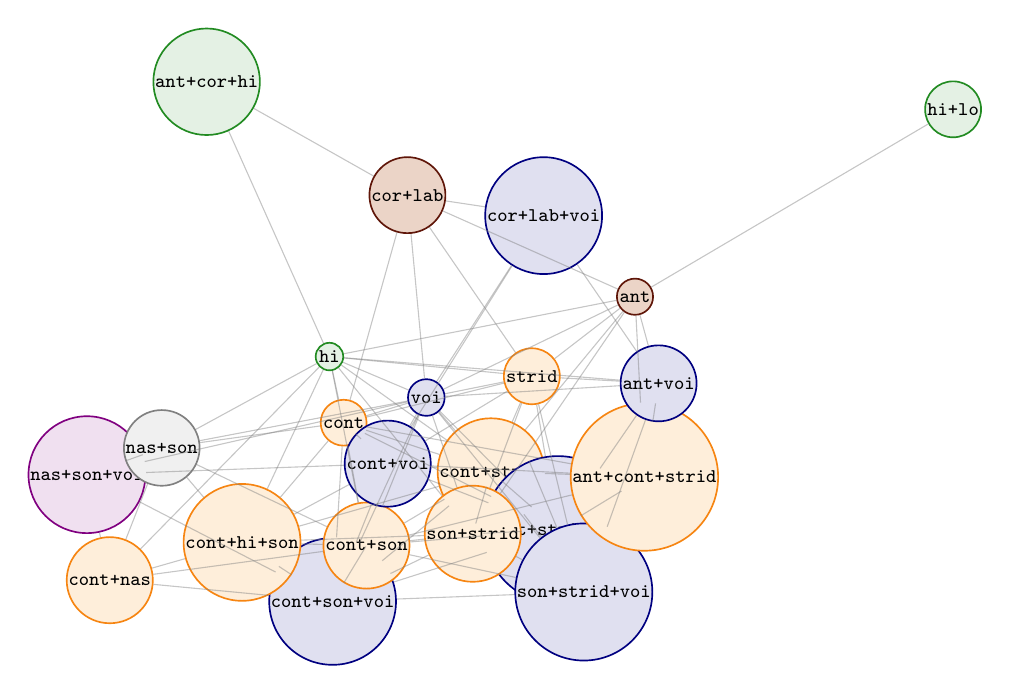
\begin{tikzpicture}[font=\scriptsize]
\node[circle,draw=NavyBlue,fill=NavyBlue!12,line width=0.6pt,inner sep=0.5pt,minimum size=0.40cm] (P0) at (-1.19,-0.71) {\texttt{{voi}}};
\node[circle,draw=Sepia,fill=Sepia!12,line width=0.6pt,inner sep=0.5pt,minimum size=0.35cm] (P1) at (-1.43,1.86) {\texttt{{cor+lab}}};
\node[circle,draw=ForestGreen,fill=ForestGreen!12,line width=0.6pt,inner sep=0.5pt,minimum size=0.33cm] (P2) at (5.50,2.95) {\texttt{{hi+lo}}};
\node[circle,draw=Purple,fill=Purple!12,line width=0.6pt,inner sep=0.5pt,minimum size=0.33cm] (P3) at (-5.50,-1.69) {\texttt{{nas+son+voi}}};
\node[circle,draw=BurntOrange,fill=BurntOrange!12,line width=0.6pt,inner sep=0.5pt,minimum size=0.32cm] (P4) at (-0.37,-1.65) {\texttt{{cont+strid}}};
\node[circle,draw=BurntOrange,fill=BurntOrange!12,line width=0.6pt,inner sep=0.5pt,minimum size=0.30cm] (P5) at (-5.21,-3.03) {\texttt{{cont+nas}}};
\node[circle,draw=NavyBlue,fill=NavyBlue!12,line width=0.6pt,inner sep=0.5pt,minimum size=0.30cm] (P6) at (0.48,-2.39) {\texttt{{cont+strid+voi}}};
\node[circle,draw=NavyBlue,fill=NavyBlue!12,line width=0.6pt,inner sep=0.5pt,minimum size=0.29cm] (P7) at (0.30,1.60) {\texttt{{cor+lab+voi}}};
\node[circle,draw=Gray,fill=Gray!12,line width=0.6pt,inner sep=0.5pt,minimum size=0.28cm] (P8) at (-4.55,-1.35) {\texttt{{nas+son}}};
\node[circle,draw=NavyBlue,fill=NavyBlue!12,line width=0.6pt,inner sep=0.5pt,minimum size=0.25cm] (P9) at (-2.38,-3.30) {\texttt{{cont+son+voi}}};
\node[circle,draw=NavyBlue,fill=NavyBlue!12,line width=0.6pt,inner sep=0.5pt,minimum size=0.24cm] (P10) at (0.81,-3.18) {\texttt{{son+strid+voi}}};
\node[circle,draw=BurntOrange,fill=BurntOrange!12,line width=0.6pt,inner sep=0.5pt,minimum size=0.22cm] (P11) at (-2.24,-1.03) {\texttt{{cont}}};
\node[circle,draw=Sepia,fill=Sepia!12,line width=0.6pt,inner sep=0.5pt,minimum size=0.22cm] (P12) at (1.46,0.57) {\texttt{{ant}}};
\node[circle,draw=BurntOrange,fill=BurntOrange!12,line width=0.6pt,inner sep=0.5pt,minimum size=0.22cm] (P13) at (-1.95,-2.59) {\texttt{{cont+son}}};
\node[circle,draw=NavyBlue,fill=NavyBlue!12,line width=0.6pt,inner sep=0.5pt,minimum size=0.21cm] (P14) at (-1.68,-1.55) {\texttt{{cont+voi}}};
\node[circle,draw=ForestGreen,fill=ForestGreen!12,line width=0.6pt,inner sep=0.5pt,minimum size=0.20cm] (P15) at (-3.98,3.30) {\texttt{{ant+cor+hi}}};
\node[circle,draw=BurntOrange,fill=BurntOrange!12,line width=0.6pt,inner sep=0.5pt,minimum size=0.19cm] (P16) at (1.58,-1.72) {\texttt{{ant+cont+strid}}};
\node[circle,draw=BurntOrange,fill=BurntOrange!12,line width=0.6pt,inner sep=0.5pt,minimum size=0.19cm] (P17) at (-0.60,-2.44) {\texttt{{son+strid}}};
\node[circle,draw=BurntOrange,fill=BurntOrange!12,line width=0.6pt,inner sep=0.5pt,minimum size=0.18cm] (P18) at (-3.53,-2.55) {\texttt{{cont+hi+son}}};
\node[circle,draw=ForestGreen,fill=ForestGreen!12,line width=0.6pt,inner sep=0.5pt,minimum size=0.18cm] (P19) at (-2.42,-0.19) {\texttt{{hi}}};
\node[circle,draw=NavyBlue,fill=NavyBlue!12,line width=0.6pt,inner sep=0.5pt,minimum size=0.17cm] (P20) at (1.76,-0.53) {\texttt{{ant+voi}}};
\node[circle,draw=BurntOrange,fill=BurntOrange!12,line width=0.6pt,inner sep=0.5pt,minimum size=0.16cm] (P21) at (0.15,-0.44) {\texttt{{strid}}};
\draw[gray,opacity=0.45,line width=0.4pt] (P0) -- (P1);
\draw[gray,opacity=0.45,line width=0.4pt] (P0) -- (P3);
\draw[gray,opacity=0.45,line width=0.4pt] (P0) -- (P4);
\draw[gray,opacity=0.45,line width=0.4pt] (P0) -- (P6);
\draw[gray,opacity=0.45,line width=0.4pt] (P0) -- (P7);
\draw[gray,opacity=0.45,line width=0.4pt] (P0) -- (P8);
\draw[gray,opacity=0.45,line width=0.4pt] (P0) -- (P9);
\draw[gray,opacity=0.45,line width=0.4pt] (P0) -- (P10);
\draw[gray,opacity=0.45,line width=0.4pt] (P0) -- (P11);
\draw[gray,opacity=0.45,line width=0.4pt] (P0) -- (P12);
\draw[gray,opacity=0.45,line width=0.4pt] (P0) -- (P13);
\draw[gray,opacity=0.45,line width=0.4pt] (P0) -- (P14);
\draw[gray,opacity=0.45,line width=0.4pt] (P0) -- (P17);
\draw[gray,opacity=0.45,line width=0.4pt] (P0) -- (P19);
\draw[gray,opacity=0.45,line width=0.4pt] (P0) -- (P20);
\draw[gray,opacity=0.45,line width=0.4pt] (P0) -- (P21);
\draw[gray,opacity=0.45,line width=0.4pt] (P1) -- (P7);
\draw[gray,opacity=0.45,line width=0.4pt] (P1) -- (P11);
\draw[gray,opacity=0.45,line width=0.4pt] (P1) -- (P12);
\draw[gray,opacity=0.45,line width=0.4pt] (P1) -- (P15);
\draw[gray,opacity=0.45,line width=0.4pt] (P1) -- (P21);
\draw[gray,opacity=0.45,line width=0.4pt] (P2) -- (P12);
\draw[gray,opacity=0.45,line width=0.4pt] (P3) -- (P5);
\draw[gray,opacity=0.45,line width=0.4pt] (P3) -- (P8);
\draw[gray,opacity=0.45,line width=0.4pt] (P3) -- (P9);
\draw[gray,opacity=0.45,line width=0.4pt] (P3) -- (P14);
\draw[gray,opacity=0.45,line width=0.4pt] (P4) -- (P6);
\draw[gray,opacity=0.45,line width=0.4pt] (P4) -- (P9);
\draw[gray,opacity=0.45,line width=0.4pt] (P4) -- (P10);
\draw[gray,opacity=0.45,line width=0.4pt] (P4) -- (P11);
\draw[gray,opacity=0.45,line width=0.4pt] (P4) -- (P12);
\draw[gray,opacity=0.45,line width=0.4pt] (P4) -- (P13);
\draw[gray,opacity=0.45,line width=0.4pt] (P4) -- (P14);
\draw[gray,opacity=0.45,line width=0.4pt] (P4) -- (P16);
\draw[gray,opacity=0.45,line width=0.4pt] (P4) -- (P17);
\draw[gray,opacity=0.45,line width=0.4pt] (P4) -- (P18);
\draw[gray,opacity=0.45,line width=0.4pt] (P4) -- (P19);
\draw[gray,opacity=0.45,line width=0.4pt] (P4) -- (P21);
\draw[gray,opacity=0.45,line width=0.4pt] (P5) -- (P8);
\draw[gray,opacity=0.45,line width=0.4pt] (P5) -- (P9);
\draw[gray,opacity=0.45,line width=0.4pt] (P5) -- (P13);
\draw[gray,opacity=0.45,line width=0.4pt] (P5) -- (P18);
\draw[gray,opacity=0.45,line width=0.4pt] (P5) -- (P19);
\draw[gray,opacity=0.45,line width=0.4pt] (P6) -- (P9);
\draw[gray,opacity=0.45,line width=0.4pt] (P6) -- (P10);
\draw[gray,opacity=0.45,line width=0.4pt] (P6) -- (P11);
\draw[gray,opacity=0.45,line width=0.4pt] (P6) -- (P13);
\draw[gray,opacity=0.45,line width=0.4pt] (P6) -- (P14);
\draw[gray,opacity=0.45,line width=0.4pt] (P6) -- (P16);
\draw[gray,opacity=0.45,line width=0.4pt] (P6) -- (P17);
\draw[gray,opacity=0.45,line width=0.4pt] (P6) -- (P20);
\draw[gray,opacity=0.45,line width=0.4pt] (P6) -- (P21);
\draw[gray,opacity=0.45,line width=0.4pt] (P7) -- (P14);
\draw[gray,opacity=0.45,line width=0.4pt] (P7) -- (P20);
\draw[gray,opacity=0.45,line width=0.4pt] (P8) -- (P11);
\draw[gray,opacity=0.45,line width=0.4pt] (P8) -- (P13);
\draw[gray,opacity=0.45,line width=0.4pt] (P8) -- (P18);
\draw[gray,opacity=0.45,line width=0.4pt] (P8) -- (P19);
\draw[gray,opacity=0.45,line width=0.4pt] (P9) -- (P10);
\draw[gray,opacity=0.45,line width=0.4pt] (P9) -- (P11);
\draw[gray,opacity=0.45,line width=0.4pt] (P9) -- (P13);
\draw[gray,opacity=0.45,line width=0.4pt] (P9) -- (P14);
\draw[gray,opacity=0.45,line width=0.4pt] (P9) -- (P17);
\draw[gray,opacity=0.45,line width=0.4pt] (P9) -- (P18);
\draw[gray,opacity=0.45,line width=0.4pt] (P10) -- (P13);
\draw[gray,opacity=0.45,line width=0.4pt] (P10) -- (P17);
\draw[gray,opacity=0.45,line width=0.4pt] (P10) -- (P20);
\draw[gray,opacity=0.45,line width=0.4pt] (P10) -- (P21);
\draw[gray,opacity=0.45,line width=0.4pt] (P11) -- (P13);
\draw[gray,opacity=0.45,line width=0.4pt] (P11) -- (P14);
\draw[gray,opacity=0.45,line width=0.4pt] (P11) -- (P16);
\draw[gray,opacity=0.45,line width=0.4pt] (P11) -- (P18);
\draw[gray,opacity=0.45,line width=0.4pt] (P11) -- (P19);
\draw[gray,opacity=0.45,line width=0.4pt] (P11) -- (P21);
\draw[gray,opacity=0.45,line width=0.4pt] (P12) -- (P16);
\draw[gray,opacity=0.45,line width=0.4pt] (P12) -- (P17);
\draw[gray,opacity=0.45,line width=0.4pt] (P12) -- (P19);
\draw[gray,opacity=0.45,line width=0.4pt] (P12) -- (P20);
\draw[gray,opacity=0.45,line width=0.4pt] (P12) -- (P21);
\draw[gray,opacity=0.45,line width=0.4pt] (P13) -- (P14);
\draw[gray,opacity=0.45,line width=0.4pt] (P13) -- (P16);
\draw[gray,opacity=0.45,line width=0.4pt] (P13) -- (P17);
\draw[gray,opacity=0.45,line width=0.4pt] (P13) -- (P18);
\draw[gray,opacity=0.45,line width=0.4pt] (P13) -- (P19);
\draw[gray,opacity=0.45,line width=0.4pt] (P14) -- (P16);
\draw[gray,opacity=0.45,line width=0.4pt] (P14) -- (P18);
\draw[gray,opacity=0.45,line width=0.4pt] (P14) -- (P21);
\draw[gray,opacity=0.45,line width=0.4pt] (P15) -- (P19);
\draw[gray,opacity=0.45,line width=0.4pt] (P16) -- (P20);
\draw[gray,opacity=0.45,line width=0.4pt] (P17) -- (P18);
\draw[gray,opacity=0.45,line width=0.4pt] (P17) -- (P19);
\draw[gray,opacity=0.45,line width=0.4pt] (P17) -- (P21);
\draw[gray,opacity=0.45,line width=0.4pt] (P18) -- (P19);
\draw[gray,opacity=0.45,line width=0.4pt] (P19) -- (P20);
\draw[gray,opacity=0.45,line width=0.4pt] (P19) -- (P21);
\draw[gray,opacity=0.45,line width=0.4pt] (P20) -- (P21);
\end{tikzpicture}
\caption{\textbf{Operator graph $G_O$ of Indo-European.} Nodes are operators (the 22 with highest support), sized by frequency and coloured by change type (\textcolor{NavyBlue}{voicing}, \textcolor{BurntOrange}{fricativization}, \textcolor{ForestGreen}{palatalization/height}, \textcolor{Sepia}{place}, \textcolor{Purple}{prenasalization}). An edge joins $u,v$ when their composition $u\oplus v$ is itself an operator of the repertoire --- so this is the graph of \emph{additive closure}. Dense connectivity is the visual face of the composition index $C(O)$.}
\end{figure}
